% Define the document as a subfile and reference its root.
\documentclass[../main.tex]{subfiles}

% Begin the document.
\begin{document}
\appendix
    \chapter{Participants' Information Sheet \& Consent Form} \label{app:consent}
        The following pages contain the participants' information sheet and consent
            form, verbatim as presented to participants.

        \begin{center}
            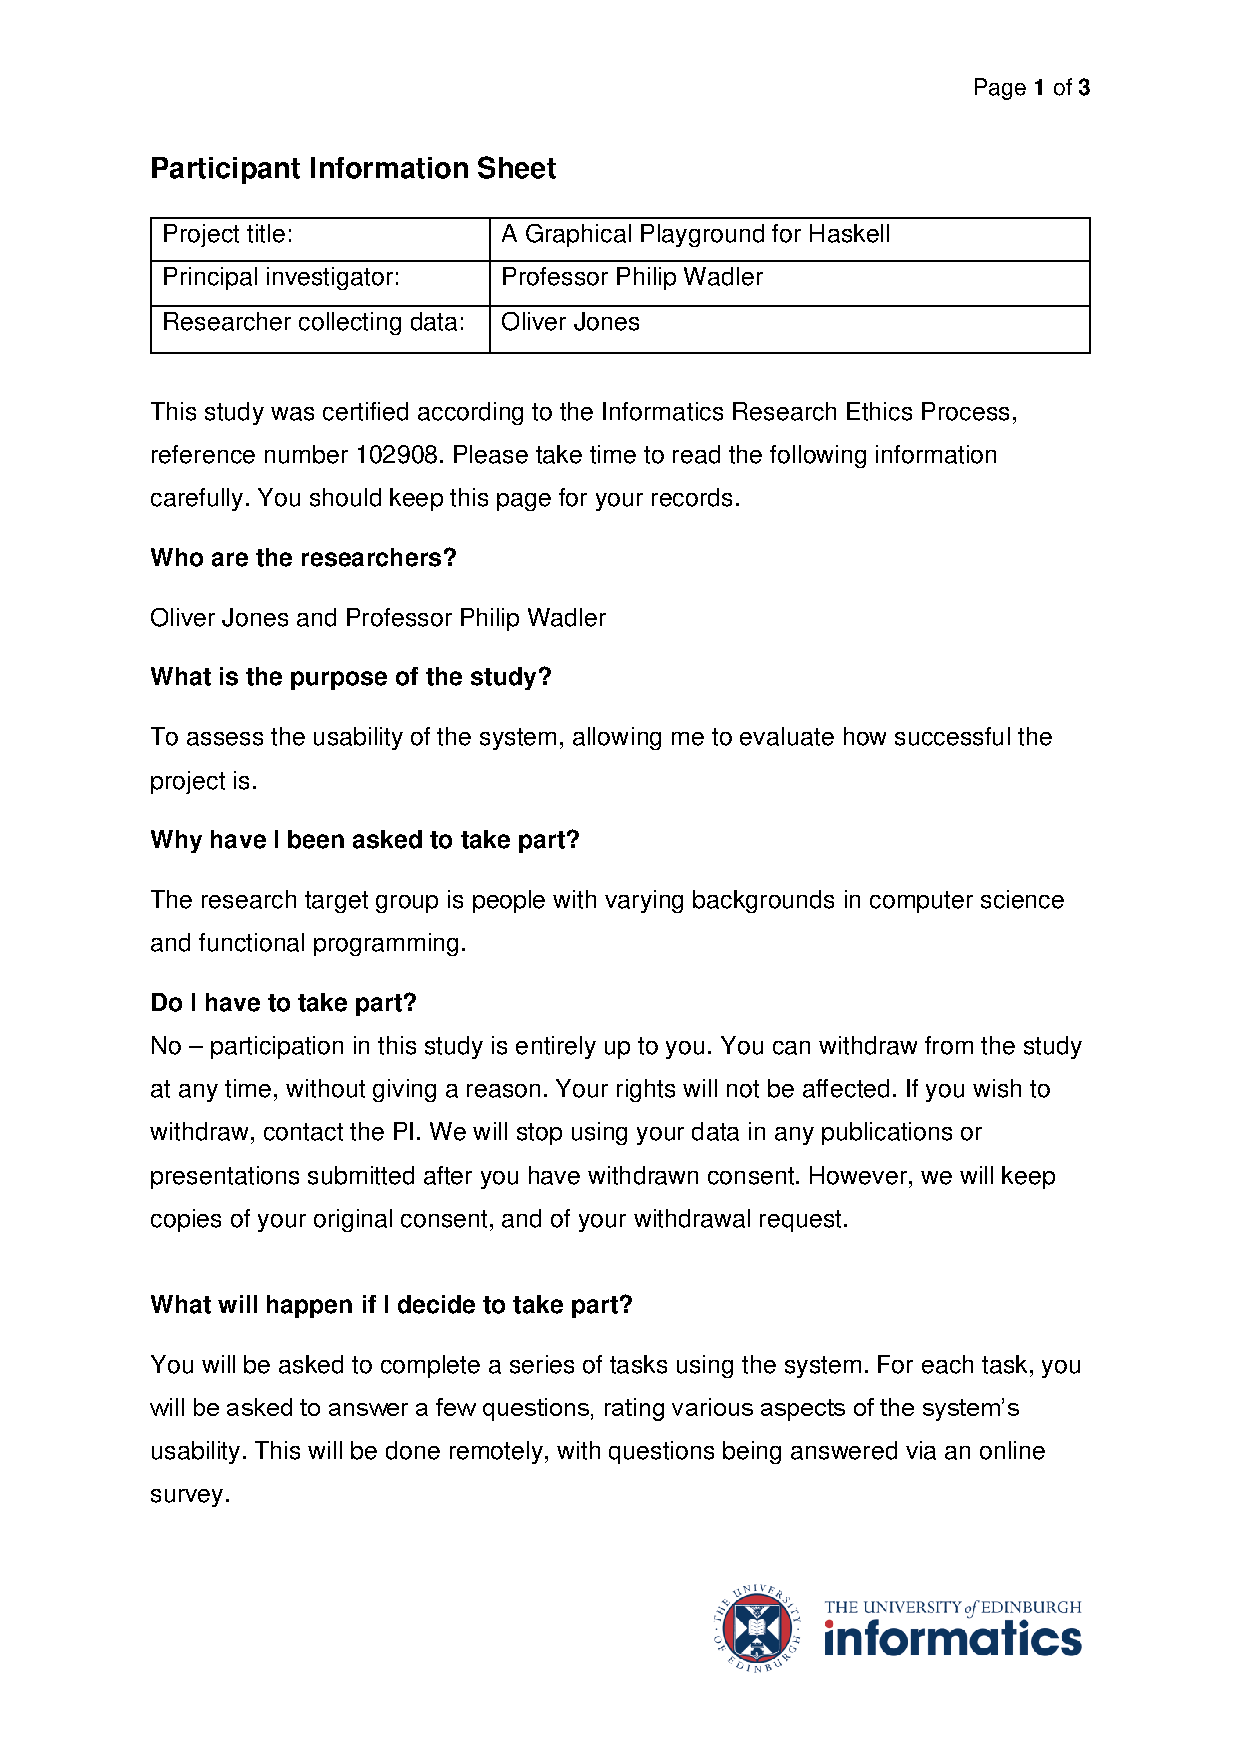
\includepdf[pages=-]{participant-information.pdf}
        \end{center}

    \chapter{Responses to User Testing \& Feedback Survey} \label{app:feedback}
        The following pages contain the tabulated quantitative responses to the user
            testing and feedback survey.

        \section*{Writing a Basic Haskell Program}
            \begin{table}[H]
                \centering
                \begin{tabular}{c|c|c|c}
                    \textbf{Qualifications} & \textbf{Experience} & \textbf{Ease of Task} & \textbf{Time Taken} \\
                    \hline
                    Bachelor's Degree       & Intermediate        & 7                     & 1-5 minutes         \\
                    Bachelor's Degree       & Intermediate        & 10                    & 1-5 minutes         \\
                    Postgraduate Degree     & Advanced            & 10                    & less than a minute  \\
                    A-Level or equivalent   & Intermediate        & 2                     & 11-15 minutes       \\
                    A-Level or equivalent   & Beginner            & 2                     & 11-15 minutes       \\
                    A-Level or equivalent   & Beginner            & 2                     & 16-20 minutes       \\
                    Bachelor's Degree       & Intermediate        & 8                     & 1-5 minutes         \\
                    Postgraduate Degree     & Advanced            & 10                    & less than a minute  \\
                    Other                   & Intermediate        & 10                    & 1-5 minutes         \\
                    Bachelor's Degree       & Intermediate        & 8                     & 1-5 minutes         \\
                    Bachelor's Degree       & Beginner            & 4                     & 6-10 minutes        \\
                \end{tabular}
                \caption{The results of the first task}
            \end{table}
        \section*{Producing a Simple Graphic Using the Reference Page}
            \begin{table}[H]
                \centering
                \begin{tabular}{c|c|c|c|c}
                    \textbf{Qualifications} & \textbf{Experience}
                                            & \makecell{\textbf{Ease of}                             \\ \textbf{Task}}
                                            & \makecell{\textbf{Quality of}                          \\ \textbf{Docs}}
                                            & \textbf{Time Taken}                                    \\
                    \hline
                    Bachelor's Degree       & Intermediate                  & 4  & 5 & 6-10 minutes  \\
                    Bachelor's Degree       & Intermediate                  & 10 & 9 & 11-15 minutes \\
                    Postgraduate Degree     & Advanced                      & 6  & 6 & 6-10 minutes  \\
                    A-Level or equivalent   & Intermediate                  & 2  & 3 & 6-10 minutes  \\
                    A-Level or equivalent   & Beginner                      & 4  & 3 & 11-15 minutes \\
                    A-Level or equivalent   & Beginner                      & 1  & 4 & 11-15 minutes \\
                    Bachelor's Degree       & Intermediate                  & 5  & 3 & 6-10 minutes  \\
                    Postgraduate Degree     & Advanced                      & 9  & 9 & 6-10 minutes  \\
                    Other                   & Intermediate                  & 8  & 7 & 1-5 minutes   \\
                    Bachelor's Degree       & Intermediate                  & 6  & 8 & 6-10 minutes  \\
                    Bachelor's Degree       & Beginner                      & 5  & 8 & 11-15 minutes \\
                \end{tabular}
                \caption{The results of the second task, including the quality of the documentation}
            \end{table}
        \section*{Altering a Pre-existing Program to Produce a Different Image}
            \begin{table}[H]
                \centering
                \begin{tabular}{c|c|c|c}
                    \textbf{Qualifications} & \textbf{Experience} & \textbf{Ease of Task} & \textbf{Time Taken} \\
                    \hline
                    Bachelor's Degree       & Intermediate        & 9                     & less than a minute  \\
                    Bachelor's Degree       & Intermediate        & 9                     & 1-5 minutes         \\
                    Postgraduate Degree     & Advanced            & 6                     & 6-10 minutes        \\
                    A-Level or equivalent   & Intermediate        & 10                    & 1-5 minutes         \\
                    A-Level or equivalent   & Beginner            & 10                    & 1-5 minutes         \\
                    A-Level or equivalent   & Beginner            & 9                     & less than a minute  \\
                    Bachelor's Degree       & Intermediate        & 8                     & 1-5 minutes         \\
                    Postgraduate Degree     & Advanced            & 10                    & 1-5 minutes         \\
                    Other                   & Intermediate        & 10                    & 1-5 minutes         \\
                    Bachelor's Degree       & Intermediate        & 9                     & 1-5 minutes         \\
                    Bachelor's Degree       & Beginner            & 10                    & 1-5 minutes         \\
                \end{tabular}
                \caption{The results of the third task}
            \end{table}
        \section*{Altering a Pre-existing Program to Produce a Different Animation}
            \begin{table}[H]
                \centering
                \begin{tabular}{c|c|c|c}
                    \textbf{Qualifications} & \textbf{Experience} & \textbf{Ease of Task} & \textbf{Time Taken} \\
                    \hline
                    Bachelor's Degree       & Intermediate        & 8                     & 1-5 minutes         \\
                    Bachelor's Degree       & Intermediate        & 9                     & 6-10 minutes        \\
                    Postgraduate Degree     & Advanced            & 7                     & 6-10 minutes        \\
                    A-Level or equivalent   & Intermediate        & 0                     & 1-5 minutes         \\
                    A-Level or equivalent   & Beginner            & 0                     & 21+ minutes         \\
                    A-Level or equivalent   & Beginner            & 2                     & 11-15 minutes       \\
                    Bachelor's Degree       & Intermediate        & 3                     & 6-10 minutes        \\
                    Postgraduate Degree     & Advanced            & 8                     & 1-5 minutes         \\
                    Other                   & Intermediate        & 10                    & 1-5 minutes         \\
                    Bachelor's Degree       & Intermediate        & 8                     & 1-5 minutes         \\
                    Bachelor's Degree       & Beginner            & 7                     & 6-10 minutes        \\
                \end{tabular}
                \caption{The results of the fourth task}
            \end{table}
        \section*{Overall Ratings}
            \begin{table}[H]
                \centering
                \begin{tabular}{c|c|c}
                    \textbf{Qualifications} & \textbf{Experience} & \textbf{Rating} \\
                    \hline
                    Bachelor's Degree       & Intermediate        & 5               \\
                    Bachelor's Degree       & Intermediate        & 4               \\
                    Postgraduate Degree     & Advanced            & 4               \\
                    A-Level or equivalent   & Intermediate        & 3               \\
                    A-Level or equivalent   & Beginner            & 3               \\
                    A-Level or equivalent   & Beginner            & 3               \\
                    Bachelor's Degree       & Intermediate        & 4               \\
                    Postgraduate Degree     & Advanced            & 5               \\
                    Other                   & Intermediate        & 5               \\
                    Bachelor's Degree       & Intermediate        & 5               \\
                    Bachelor's Degree       & Beginner            & 4               \\
                \end{tabular}
                \caption{The overall ratings of the website, out of 5}
            \end{table}

    \chapter{Graphics Library Code Listings} \label{app:code}
        The following pages contain the code listings for the full graphics library.
        \section*{\texttt{Lib.hs}}
            \lstinputlisting[language={Haskell}]{../public/lib/Lib.hs}
        \section*{\texttt{Internal.hs}}
            \lstinputlisting[language={Haskell}]{../public/lib/Internal.hs}
        \section*{\texttt{Canvas.hs}}
            \lstinputlisting[language={Haskell}]{../public/lib/Canvas.hs}
        \section*{\texttt{Shape.hs}}
            \lstinputlisting[language={Haskell}]{../public/lib/Shape.hs}
        \section*{\texttt{Maths.hs}}
            \lstinputlisting[language={Haskell}]{../public/lib/Maths.hs}
        \section*{\texttt{Color.hs}}
            \lstinputlisting[language={Haskell}]{../public/lib/Color.hs}
\end{document}
